% !TeX root = Protokoll.tex
\subsection{Das Hohlleiter Feld}
Hohlleiter sind Rohre, die meistens Rechteckig geformt sind, diese können auch andere Geometrien aufweisen können. In einem Hohlleiter werden Energien mit hohen Frequenzen transportiert. Die elektromagnetische Welle kann viele verschiedene Moden transportieren. Diese lassen sich kategorisieren, in die transversale elektrische Mode (TE-Mode), in die transversale magnetische Mode (TM-Mode) oder in die transversale elektromagnetische Mode (TEM-Mode). Hier ist der namens gebende teil Senkrecht zur Ausbreitungsrichtung der Welle. Für jede Mode gibt es eine untere Frequenz unterhalb der keine Energie mehr übertragen wird, die sogenannte cut-off-Frequenz.

\subsection{Reflexklystrons}
\begin{figure}[h!]
\centering
	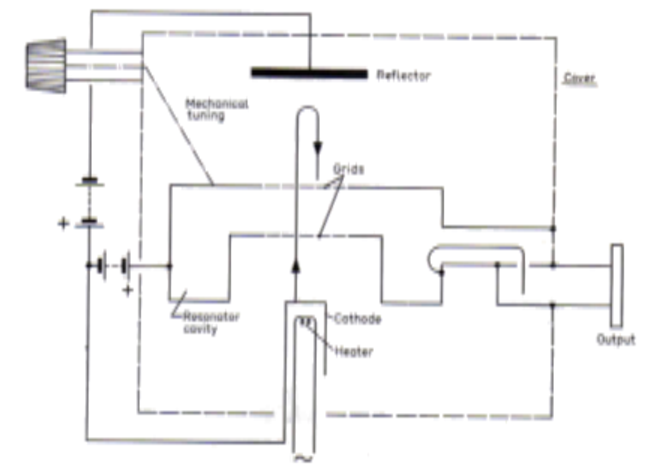
\includegraphics[angle = 1 , scale = 0.8]{../Grafiken/Klystron_Schema3.pdf}
	\caption{Schematischer Aufbau eines Reflexklystrons.\cite{V53}}\label{fig:RefKlystron}
\end{figure}
Unter einem Klystron versteht sich eine Mikrowellenröhre, die durch Geschwindigkeitsmodulation von Elektronen Mikrowellenenergie erzeugt. In \cref{fig:RefKlystron} wird der schematische Aufbau eines Reflexklystrons dargestellt. Aus der Kathode lösen sich Elektronen und werden vom Positiven Resonator beschleunigt und durch laufen diesen. Der Reflektor hat ein negatives Potential und reflektiert die Elektronen. Deshalb durchlaufen sie erneut den Resonator. Wenn das Feld zwischen den Resonatorgittern oszilliert, entsteht ein Hohlleiter Feld im Resonator. Die Elektronen werden dadurch zu Bündeln gepackt. Wenn ein Bündel zu einer Zeit im Resonator ist, wo sie beschleunigt werden, dann 